\documentclass[]{tukediphc}
%% -----------------------------------------------------------------
%% tento subor ma kodovanie utf-8
%%
%% na kompilaciu pouzivajte format pdfcslatex 
%%
%% vytvorene distribuciou texlive 2009-7, OS GNU/Linux
%% vytvorene distribuciou TeXLive 2010, OS Win XP
%% februar 2013
%% -----------------------------------------------------------------
\usepackage[utf8]{inputenc}
%\usepackage[T1]{fontenc}
\usepackage{lmodern,textcase}
\usepackage[slovak]{babel}\renewcommand{\figurename}{Obr\'azok}
\def\refname{Zoznam pou\v{z}itej literat\'ury}
\usepackage{latexsym}
\usepackage{dcolumn} % zarovnanie cisiel v tabulke podla des. ciarky
\usepackage{hhline}
\usepackage{amsmath}
\usepackage{subfig}
\usepackage{nicefrac} % pekne zlomky
\usepackage{upgreek} % napr. $\upmu\mathrm{m}$ pre mikrometer ...
\usepackage[final]{showkeys}%color%notref%notcite%final
\usepackage[slovak,noprefix]{nomencl}
\makeglossary % prikaz na vytvorenie suboru .glo
\usepackage{parskip}% 'zhusti' polozky obsahu
%%
%\usepackage[dvips]{graphicx}
%\DeclareGraphicsExtensions{.eps}
\usepackage[pdftex]{graphicx}
\DeclareGraphicsExtensions{.pdf,.png,.jpg,.mps}
\graphicspath{{figures/}} % priecinok na obrazky
%%
%% Cislovane citovanie
%\usepackage[numbers]{natbib}
%%
%% Citovanie podľa mena autora a roku
\usepackage{natbib} %\citestyle{chicago}
% -----------------------------------------------------------------
%% tlač !!!
\usepackage[pdftex,unicode=true,bookmarksnumbered=true,
bookmarksopen=true,pdfmenubar=true,pdfview=Fit,linktocpage=true,
pageanchor=true,bookmarkstype=toc,pdfpagemode=UseOutlines,
pdfstartpage=1]{hyperref}
\hypersetup{%
baseurl={http://www.tuke.sk/sevcovic},
pdfcreator={pdfcsLaTeX},
pdfkeywords={Riadenie procesov, Oceliarstvo, Vizualizácia, Virtuálna realita, Matematické modelovanie},
pdftitle={Písomná príprava k predmetu Informačné technológie v riadení procesov},
pdfauthor={Michal Takáč},
pdfsubject={Dizertačná skúška}
} 
%% nehodiace zakomentujte !
%\dippraca{Elaborát z predmetu Riadenie procesov}
%\bakpraca{Príprava na dizertačnú skúšku}
%%
\nazov{Písomná príprava k predmetu Informačné technológie v riadení procesov}
%% ked praca nema 'podnazov' zakomentujte nasledujuci riadok
%% alebo polozku nechajte prazdnu
\podnazov{}
\autor{Ing.~Michal Takáč}
\veduciprace{doc.~Ing.~Ján~Kačur, PhD.}
\univerzita{Technická univerzita v~Košiciach}
\fakulta{Fakulta baníctva, ekológie, riadenia a geotechnológií}
\skratkafakulty{FBERG}
\katedra{Ústav riadenia a informatizácie výrobných procesov}
\skratkakatedry{URIVP}
\odbor{Riadenie procesov}
\specializacia{Kybernetika}
\abstrakt{Abstrakt je povinnou súčasťou každej práce. Je výstižnou
charakteristikou obsahu dokumentu. Nevyjadruje hodnotiace stanovisko
autora. Má byť\/ taký informatívny, ako to povoľuje podstata práce.
Text abstraktu sa píše ako jeden odstavec. Abstrakt neobsahuje odkazy
na samotný text práce. Mal by mať\/ rozsah 250 až 500 slov. Pri
štylizácii sa používajú celé vety, slovesá v činnom rode a tretej
osobe. Používa sa odborná terminológia, menej zvyčajné termíny,
skratky a~symboly sa pri prvom výskyte v texte definujú.}
\klucoveslova{Riadenie procesov, Oceliarstvo, Vizualizácia, Virtuálna realita, Matematické modelovanie}
\datumodovzdania{29. 5. 2020}
\mesto{Košice}

\begin{document}
\renewcommand\theHfigure{\theHsection.\arabic{figure}}
\renewcommand\theHtable{\theHsection.\arabic{table}}
\bibliographystyle{dcu}

\prvastrana


\thispagestyle{empty}
\tableofcontents
\newpage
%
%\thispagestyle{empty}
%%\addcontentsline{toc}{section}{\numberline{}Zoznam obrázkov}
%\listoffigures
%\newpage
%
%\thispagestyle{empty}
%%\addcontentsline{toc}{section}{\numberline{}Zoznam tabuliek}
%\listoftables
%\newpage

%%%%%%%%%%%%%%%%%%%%%%%%%%%%%%%%%

\setcounter{page}{1}
\setcounter{equation}{0}
\setcounter{figure}{0}
\setcounter{table}{0}

\section{Úvod}

Cieľom riadenia procesu je udržiavať kľúčové parametre prevádzky procesu v úzkom rozmedzí referenčnej hodnoty alebo požadovanej hodnoty. Niekdajšiu potrebu riadiť túto činnosť manuálne v súčasnej dobe nahrádzajú programovateľné automaty a regulátory v snahe ovládať premennú automatizovane. Jednoduchý regulátor môže udržiavať procesnú veličinu v slučke na rovnomernej úrovni, pokiaľ nedôjde k nadmernému rušeniu. Pri komplexných procesoch, ako sú tie v metalurgii, sa využívajú desiatky až stovky takýchto regulátorov, niektoré s integrovanými LCD panelmi \citep{Al-Megren2016}.

Informačné systémy v procesnom riadení sú implementované pre rôzne škály riadiacich systémov, ktoré môže tvoriť niekoľko menších modulárnych panelových automatov až po veľké, vzájomne prepojené a interaktívne distribuované riadiace systémy s mnohými tisíckami prevádzkových pripojení.

Najjednoduchšie riadiace systémy sú založené na malých diskrétnych regulátoroch, z ktorých každý má jednu regulačnú slučku. Zvyčajne sú namontované na panel, ktorý umožňuje priame odčítanie hodnôt z predného panela a poskytuje prostriedky na manuálny zásah operátora, a to buď na manuálne riadenie procesu, alebo na zmenu požadovaných riadiacich hodnôt.

\section{Monitorovanie a zber dát}

Za účelom monitorovania a riadenia procesu je možné využiť rôzne meracie systémy na poskytnutie spätnej väzby operátorovi alebo priamo existujúcemu systému na automatizované riadenie. Tieto merania môžu byť priame alebo nepriame, ako aj~s~časovým oneskorením alebo bez neho \cite{Widlund1998}.

Na výrobných linkách sa častokrát vykonáva veľké množstvo meraní. Sledujú sa nimi zmeny meranej veličiny (fyzikálnej alebo chemickej, napr. tlak, prietok, hustota, kyslosť, rýchlosť, napätie, teplota, hmotnosť atď.). Dáta sú získavané zo snímačov (senzorov), ktoré reagujú na túto zmenu, a to buď okamžite alebo s sa zameriavajú na časový priebeh zmeny. Snímače môžu taktiež sledovať polohu ventilu alebo stav uzatvorenia nejakého otvoru (zátka fľaše, menič prietoku). Snímače zobrazujú hodnoty meranej veličiny buď priamo (odmerka, ortuťový teplomer) alebo sú spojené s indikátorom. Sú väčšinou elektrické, čo znamená, že transformujú informáciu o meranej veličine na elektrický signál, čím umožňujú transformáciu aj neelektrickej veličiny. Pre spracovanie elektrického signálu zo snímača na počítači je potrebné využitie prevodníka, ktorý prevedie analógový signál na digitálny.

Keďže cieľom výroby ocele v kyslíkových konvertoroch je spálenie (tzv. oxidácia) nežiadúcich nečistôt obsiahnutých v kovovej vsádzke, účelom tohto oxidačného procesu teda je:

\begin{itemize}
	\item znížiť obsah uhlíka na predpísanú úroveň (z približne 4 \% na menej ako 1 \%, ale často nižšie),
	\item upraviť obsah potrebných cudzích prvkov,
	\item odstrániť nežiadúce nečistoty v maximálne možnej miere.
\end{itemize}

Následnou úlohou riadiaceho procesu je potom získanie predpísaných parametrov ocele, ktorá sa odpichuje z konvertora, vrátane hmotnosti, teploty a obsahu každého prvku. Na základe týchto parametrov sa rozhoduje o tom, či je roztavená oceľ prijateľná alebo nie. Na ich získanie a meranie je v kyslíkovom konvertore dôležitým meracím nástrojom odberná sonda. Tá poskytuje operátorovi cenné informácie o procese tavby akými sú teplota taveniny a jej zloženie. Zavádza sa automatizovane do vnútra konvertora cez horný alebo bočný otvor kým je teleso konvertora v zvislej polohe, a to 2-krát počas tavby bez nutnosti jej prerušenia. Prvé zavedenie sondy zväčša býva po vyfúkaní 90\% objemu kyslíka vyčleneného pre danú tavbu, kedy sa meria teplota, objem uhlíka, zloženie trosky, výška oceľového kúpeľa a úrovne trosky. Druhé zavedenie sa uskutočňuje po procese fúkania.

\begin{figure}[!ht]
	\centering
	\subfloat[Odberná sonda od Berry Metal Company \citep{berrymetal}.]{{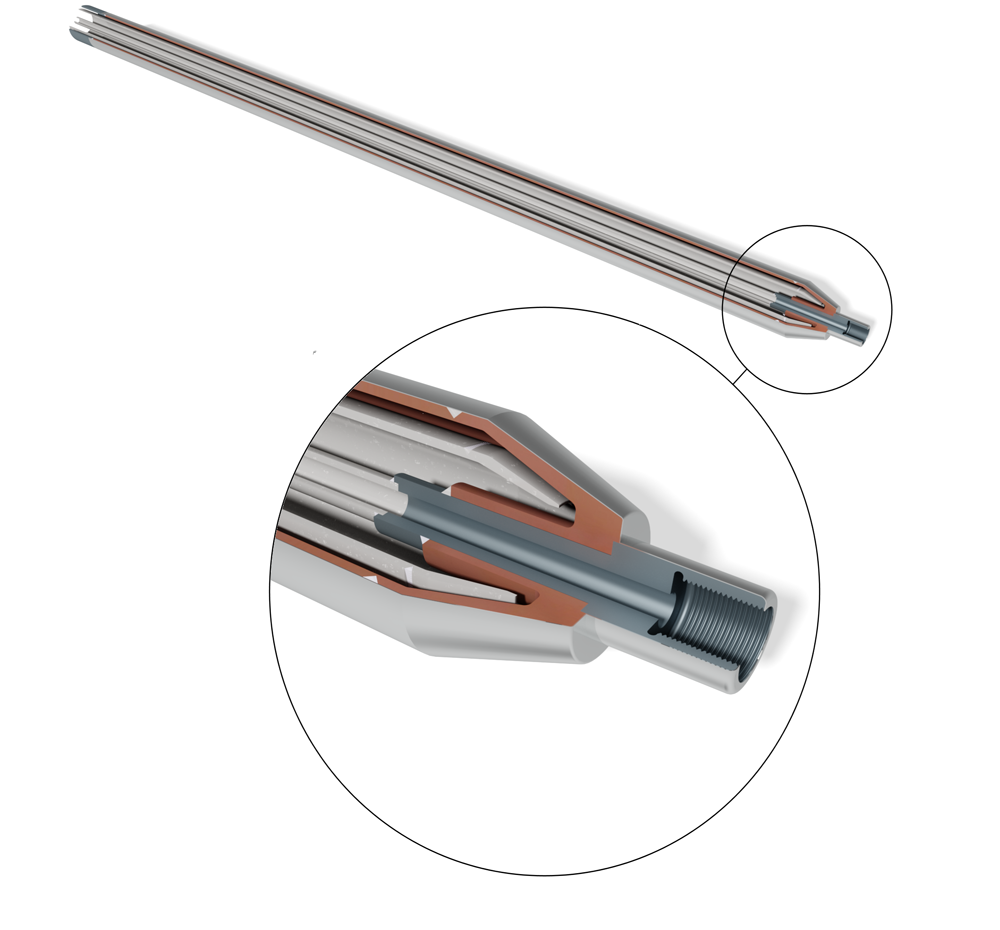
\includegraphics[width=6.5cm]{figures/sub-lance-berry.png} }}%
	\qquad
	\subfloat[Odber vzorky taveniny odbernou sondou v praxi.]{{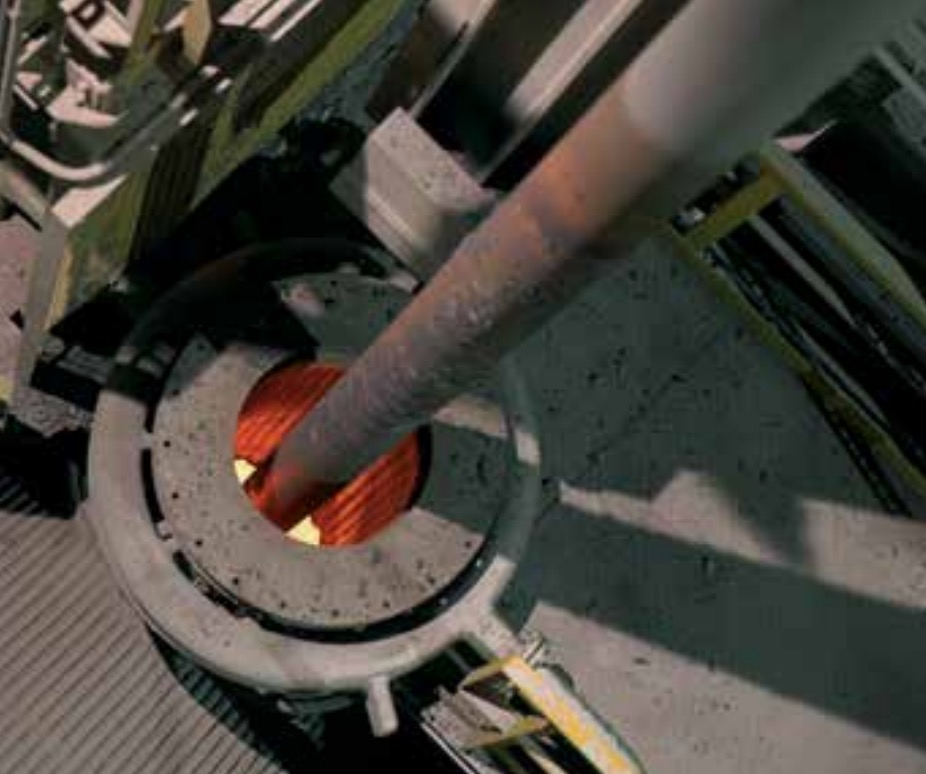
\includegraphics[width=7.35cm]{figures/sublance.jpg} }}
	\caption{Odberná sonda.}
\end{figure}

Moderné konvertory prevádzkujú merania odbernými sondami v spojení s kombinovaným statickým a dynamickým modelom riadenia procesu (SDM). Informácie získané z odbernej sondy sú ďalej spracované riadiacim systémom, ktorého optimalizačný model sa v konečnom dôsledku snaží o zvýšenie produkcie a dosiahnutie požadovaných vlastností ocele.

\section{SCADA}

SCADA (z anglického "Supervisory Control and Data Acquisition") je softvérový systém pre správu dát, riadenie a monitorovanie priemyselných procesov, ktorý je prevádzkovaný na vyššej úrovni nad hardvérom (PLC, I/O moduly, senzory, merače, atď). SCADA systémy sprostredkovávajú konektivitu medzi technologickými procesmi, z ktorých zberajú dáta. Komunikácia s okolitým prostredím prebieha prostredníctvom štandardizovaných komunikačných protokolov (Modbus, S7, SNMP, BACnet, atď) cez priemyslové linky RS-232, RS-485, Profibus, ako aj klasickou počítačovou sieťou Ethernet. Ukladanie zbieraných dát je prevádzané od jednoduchého zápisu do textových súborov až po databázové servery (SQL/NoSQL). Vďaka štandardom, modularite a podpore všeobecne využívaných databázových systémov sa dajú SCADA systémy dobre škálovať. Môžu teda byť využíté na spracovanie veľkého množstva dát, od pár vstupných premenných až po státisíce.

Využitie si SCADA systémy našli v priemyselných odvetviach, kde je vysoký nárok na správny, bezproblémový priebeh procesov a veľký objem spracovaných dát, napr. elektrárne, teplárne, rozvodne, výmenníkové stanice, výrobné linky, chemické podniky, baliarne, skladové systémy, čističky odpadových vôd, atď. Zároveň sa využívajú častejšie aj mimo priemyslu, a to napríklad v systémoch "chytrých" domov (smart houses).

Vývoj SCADA systémov prešiel štyrmi generáciami:

\begin{enumerate}
	\item{V prvej generácii šlo o nákladné, jednoúčelové systémy, bez komunikačných sieťových služieb, takže SCADA systémy sa skladali zo samostatných systémov, ktoré neboli prepojené s inými systémami. Väčšinou v tejto dobe boli implementované na veľkých centrálnych počítačoch (PDP-11 a pod.)}
	\item{Druhá generácia priniesla podporu komunikačných protokolov (proprietárnych) čo malo za následok prepojenie jednotlivých systémov cez LAN a prenos informácií takmer v reálnom čase. Bezpečnosť systémov bola v začiatkoch prehliadaná.}
	\item{Tretia generácia stavala na rozmachu počítačových sietí, kedy vznikali otvorené komunikačné protokoly. Komplexné SCADA systémy bolo možné rozdeliť na menšie a jednoduchšie komponenty, ktoré vykonávali užší set funkcií, často aj na geograficky rôznych lokalitách a medzi sebou komunikovali cez sieť pre riadenie procesov (PCN - Process Control Network).}
	\item{Štvrtú generáciu tvoria SCADA systémy s podporou webových technológií. V sieti internet môže byť prepojené takmer všetko. Tieto systémy ponúkajú vzdialený prístup a dohľad cez internet, takže operátori vie pristupovať k rozhraniu človek-proces (HMI) systému SCADA cez akékoľvek zariadenie (desktop, tablet, smartfón).}
\end{enumerate}

\subsection{Rozhranie pre riadenie procesov človekom}

Zariadenia rozhrania človek-proces (Human-Machine Interface - HMI) sú hlavné jednotky, ktoré umožňujú operátorom kontrolovať proces získavania údajov SCADA. HMI slúži ako centrálny procesor systému a umožňuje používateľom tiež regulovať a upravovať systém podľa potreby. Prevádzkovatelia používajú rozhrania HMI na interakciu so zhromaždenými údajmi prostredníctvom grafických používateľských rozhraní (GUI), zvyčajne počítačových monitorov, a na zostavovanie správ na neskoršie použitie.

\begin{figure}[!ht]
	\centering
	\subfloat[Operatíva čistenia odchádzajúceho plynu z procesu výroby ocele v konvertore, zdroj: Matrix Technologies.]{{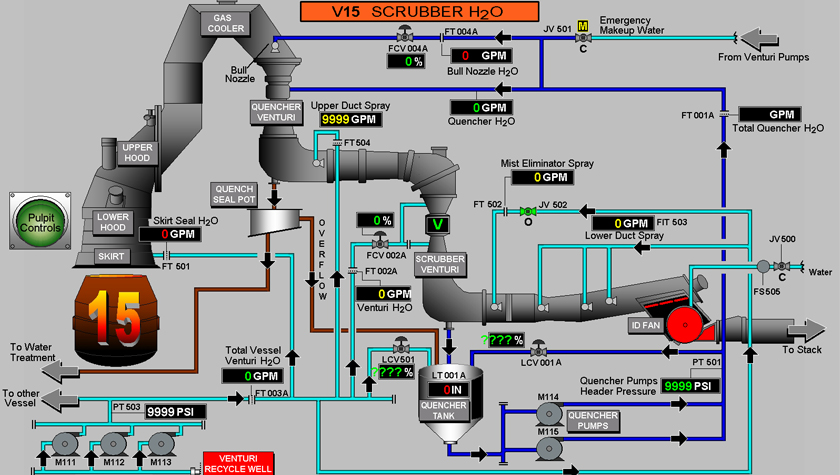
\includegraphics[width=7.1cm]{figures/bof-scada.jpg} }}%
	\qquad
	\subfloat[Odber vzorky taveniny odbernou sondou.]{{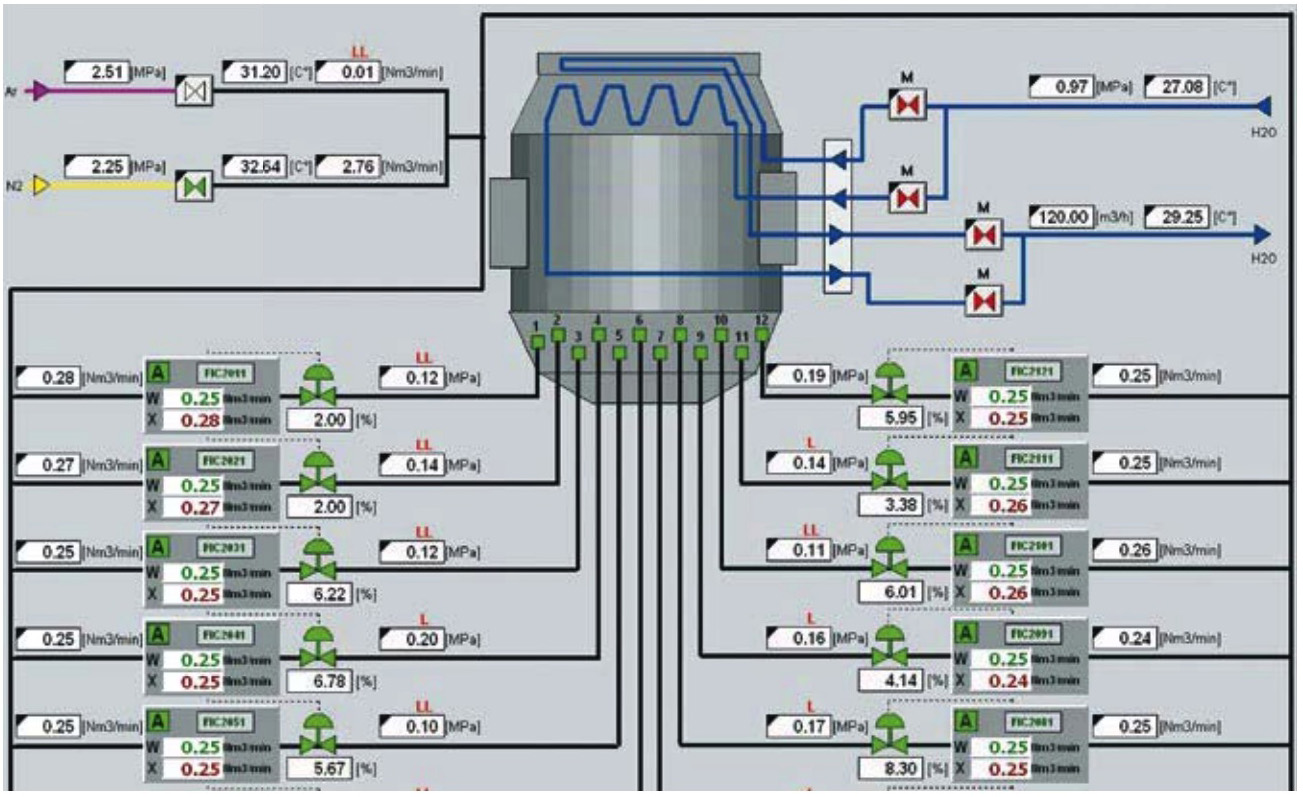
\includegraphics[width=6.65cm]{figures/bof-stirring.jpg} }}
	\caption{HMI rozhrania SCADA systémov v riadení LD procesu.}
\end{figure}

\section{Spracovanie dát}

Získané dáta môžu vyžadovať techniky predbežného spracovania, aby sa zabezpečila presná, efektívna alebo zmysluplná analýza. Čistenie dát sa týka metód zisťovania, odstraňovania a výmeny chybných alebo chýbajúcich dát. Aby sa v dátach správne identifikovali významné trendy, je potrebné nájsť kde sa nachádzajú lokálne extrémy a náhle zmeny. Dôležité je odfiltrovanie nežiadúceho šumu, na ktoré sa využívajú vyhladzovacie metódy. Metódy zoskupovania sú využívané na identifikáciu charakteristiky údajov triedenia do skupín. Často používaný softvér pre spracovanie dát je Matlab, ktorý ponúka sady nástrojov a teda odpadá nutnosť ručného programovania algoritmov. Pre väčšie prispôsobenie hardvérovým požiadavkám ako aj prípadnej potrebe vlastnej implementácie algoritmov sa využívajú programovacie jazyky Python, R alebo Lua, s veľkým množstvom predimplementovaných knižníc, ktoré je možné využiť pri programovaní vlastného riešenia spracovania údajov.

\section{Uchovanie dát}

Po analýze a spracovaní údajov zhromaždených systémom SCADA je potrebné ich uložiť na fyzicky a digitálne bezpečných miestach. Namiesto zhromažďovania a ukladania údajov ručne, SCADA automaticky zhromažďuje informácie o výrobných procesoch s časovou pečiatkou v HMI, ktoré sú kompilované do optimálneho formátu pred ich uložením do databázy. Väčšina systémov tiež používa štruktúrovaný dopytovací jazyk (SQL) alebo webové aplikácie na integráciu systémov vykonávania výroby (``Manufacturing Execution System" - MES) a systémov plánovania podnikových zdrojov (``Enterprise Resource Planning"- ERP), čo uľahčuje prevod údajov medzi rôznymi časťami siete.

Databázy v SCADA systémoch môžu byť proprietárne ale aj otvorené. Na pripojenie k nim tvorcovia SCADA softvérov ako aj vývojári tretích strán vytvárajú vlastné konektory s rozhraniami. V prípade SCADA systému od firmy Promotic je možné využívať databázy dBase, MS SQL Server, Oracle, MySQL, PostgreSQL, Microsoft Access, Excel a ďalšie, ku ktorým sa systém pripája cez technológiu ADO (ActiveX Data Objects) vytvorenou spoločnosťou Microsoft. Tá nezávisí od žiadneho backendu, avšak v súčasnosti má ADO podporu jedine cez OLE-DB, čo je aplikačné programovacie rozhranie (API), umožňujúce prístup k údajom z rôznych zdrojov.

V priemyselnom odvetví sa pri uchovaní dát poslednú dobu experimentuje aj s NoSQL databázami. NoSQL vznikla v tom čase kedy mnohé SQL databázy nedokázali zvládnuť požadovanú škálu z pohľadu nárokov na nich kladených (množstvá dát, potreba zapisovania a čítania údajov v reálnom čase). Nárast tejto novej generácie dátových služieb vyriešil mnoho problémov so škálovaním veľkých webových aplikácií a rýchlo rastúcich súborov údajov. Databázové systémy na technológii NoSQL (MongoDB) sa v posledných rokoch dostávajú aj do priemyselných oblastí, keďže ich efektívne horizontálne škálovanie (príklad: klastre desiatok až stoviek serverov v distribuovaných riadiacich systémoch) a flexibilná štruktúra ukladaných údajov prispievajú k zvládnutiu exponenciálneho nárastu spracovaných dát z internetú vecí (IoT) v dobe prechodu na novú paradigmu v priemysle s názvom Priemysel 4.0 \citep{Klingenmeier2014}.

\section{Distribuované riadiace systémy}

Distribuovaný riadiaci systém (DCS) je digitálny riadiaci systém, v ktorom sú regulátory a jednotlivé moduly systému distribuované na rôznych lokalitách. Pri väčšom počte regulačných obvodov je DCS ekonomický výhodnejší.

Jednotlivé  regulátory a hierarchie regulátorov sú v DCS prepojené komunikačnými sieťami, ktoré sú zároveň prepojené s centrálnym grafickým rozhraním no takisto môžu byť ovládané jednotlivo na jednotlivých stanovištiach pri regulátore. Tieto komunikačné siete bývajú postavené na proprietárnych ako aj otvorených komunikačných protokoloch. DCS podporujú taktiež komunikačné zbernice ako napríklad Fieldbus, PROFIBUS, HART alebo Modbus, cez ktoré tečú informačné toky vstupných a výstupných signálov, údajov, správ a chybových hlásení.

Systém SCADA sa spolieha na udržiavanie integrovaného sieťového pripojenia počas celej jeho prevádzky. Zariadenia to môžu dosiahnuť pomocou káblových aj bezdrôtových možností, pripojením prevodných jednotiek k hlavnej jednotke prostredníctvom pevnej linky alebo internetu. Väčšina zariadení má špecializované siete, na ktorých prevádzkujú svoje operácie SCADA, ktoré zabezpečujú ich systém pred rušením inými aplikáciami, ako aj proti nedovolenému vniknutiu. Zabezpečený prístup autorizovaným používateľom k správe jednotlivých zariadení zo vzdialeného miesta je možné cez priemyselné prístupové body, ktoré spravuje napr. autentifikačný server a užívateľ (pristupujúci cez internet alebo intranet) sa k HMI môže prihlásiť svojimi prihlasovacími údajmi.

\section{Komunikačné protokoly}

OPC, pôvodne ``Object Linking and Embedding for Process Control", aktuálne ale po integráciách zastrešovaných štandardov iných odvetví mimo riadenia procesov už ``Open Platform Communications" zastrešuje viacero štandardov a špecifikácií priemyselných komunikačných sietí pre otvorené pripojenie zariadení a systémov priemyselnej automatizácie. Vypracováva a držiava ich priemyselné konzorcium OPC Foundation.

OPC špecifikácie poskytujú premostenie softvérových aplikácií založených na systéme Windows a hardvér na riadenie procesov. Normy definujú konzistentné metódy prístupu k údajom zo zariadení.

\subsection{OPC UA}

OPC Unified Architecture (OPC UA) je nový komunikačný protokol (nezávislý od dodávateľa) pre aplikácie priemyselnej automatizácie. Je založený na princípe klient-server a umožňuje plynulú komunikáciu z jednotlivých senzorov a akčných členov až do ERP systému alebo cloudu. Protokol je nezávislý od platformy a má zabudované bezpečnostné mechanizmy. Pretože OPC UA je flexibilný a úplne nezávislý, považuje sa za ideálny komunikačný protokol pre implementáciu do Priemyslu 4.0.

\begin{figure}[h!]
	\centering
	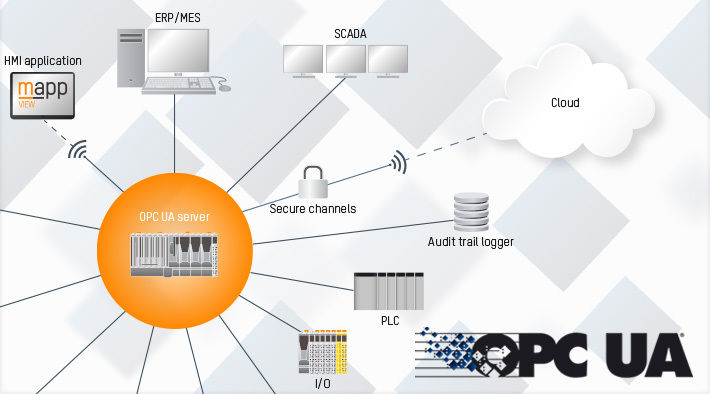
\includegraphics[width=.9\textwidth,angle=0]{figures/opc-ua.jpg}
	\caption{Grafická reprezentácia architektúry komunikačného protokolu OPC UA, zdroj: B\&R Automation.}
\end{figure}

Architektúra OPC UA predstavuje premostenie medzi komunikáciou počítačových systémov na báze IP a úrovňou výroby. Rozhrania, brány a súvisiaca strata informácií sú minulosťou, pretože všetky údaje o výrobných procesoch sa prenášajú prostredníctvom jediného protokolu - v strojoch, medzi jednotlivými strojmi alebo medzi strojom a databázou v cloude, čím odpadá nutnosť využitia rozhraní, brán medzi nekompatibilnými systémami a z tohto dôsledku možnou stratou informácií. OPC UA eliminuje potrebu tradičných systémov priemyselnej zbernice na úrovni výroby \citep{brautomation}.

Pokiaľ ide o zložité aplikácie, ako sú bezpečnosť, riadenie pohybu a komunikácia v reálnom čase, OPC UA má však svoje obmedzenia. Od rozšírenia o model publikovania a prihlásenia na odber (pub / sub) a štandardu Ethernet citlivého na čas (TSN) je však OPC UA teraz už schopná komunikovať aj v reálnom čase.

\begin{figure}[!ht]
	\centering
	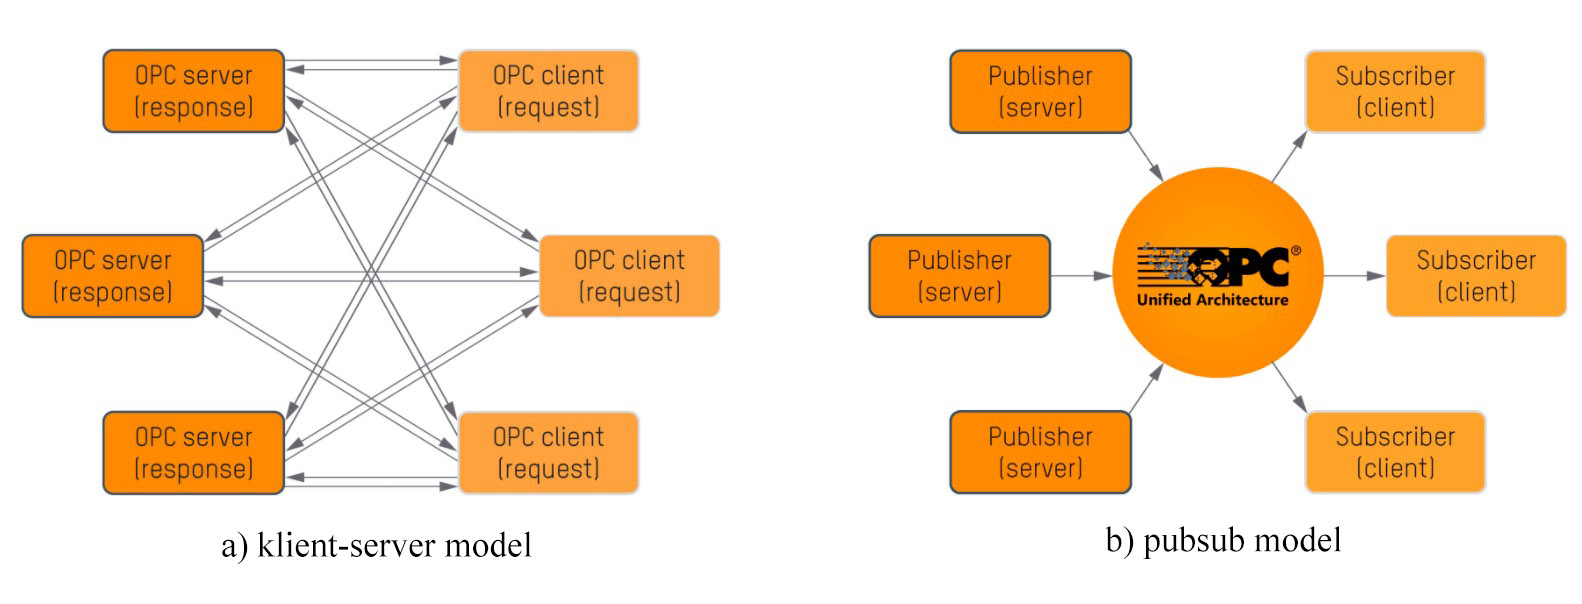
\includegraphics[width=1\textwidth,angle=0]{figures/opc-ua-pubsub.jpg}
	\caption{Rozdiel medzi architektúrou klient/server a publish/subscribe (počúvanie zmien po ju), zdroj: B\&R Automation.}
\end{figure}

\newpage

\subsection{MTConnect}

Priemyselné systémy tvorí množstvo zariadení, často od rôznych výrobcov s rôznymi konkurenčnými výhodami. Od integrácie hardvéru do uceleného riešenia výrobných systémov vo výrobných podnikoch je v súčasnosti neoddeliteľná aj časť implementácie softvérovej nadstavby. Práve schopnosť adaptovateľnosti softvéru ako informačného systému pre podporu riadenia výrobných procesov podniku udáva, do akej miery je možné architektúru systému škálovať. Táto schopnosť v priemysle závisí vo vysokej miere na štandardoch. Súčasne dostupné softvérové riešenie preto využívajú štandardizáciu údajov a dát zo zariadení, pričom počítajú s tým, že každý výrobca môže označovať tieto dáta inak.

Norma MTConnect (ANSI/MTC1.4-2018) štandardizuje údaje a dáta výrobných zariadení naprieč rôznymi výrobcami. Ponúka sémantickú slovnú zásobu pre výrobné zariadenia na poskytovanie štruktúrovaných, kontextualizovaných údajov bez proprietárneho formátu.

\begin{figure}[h!]
	\centering
	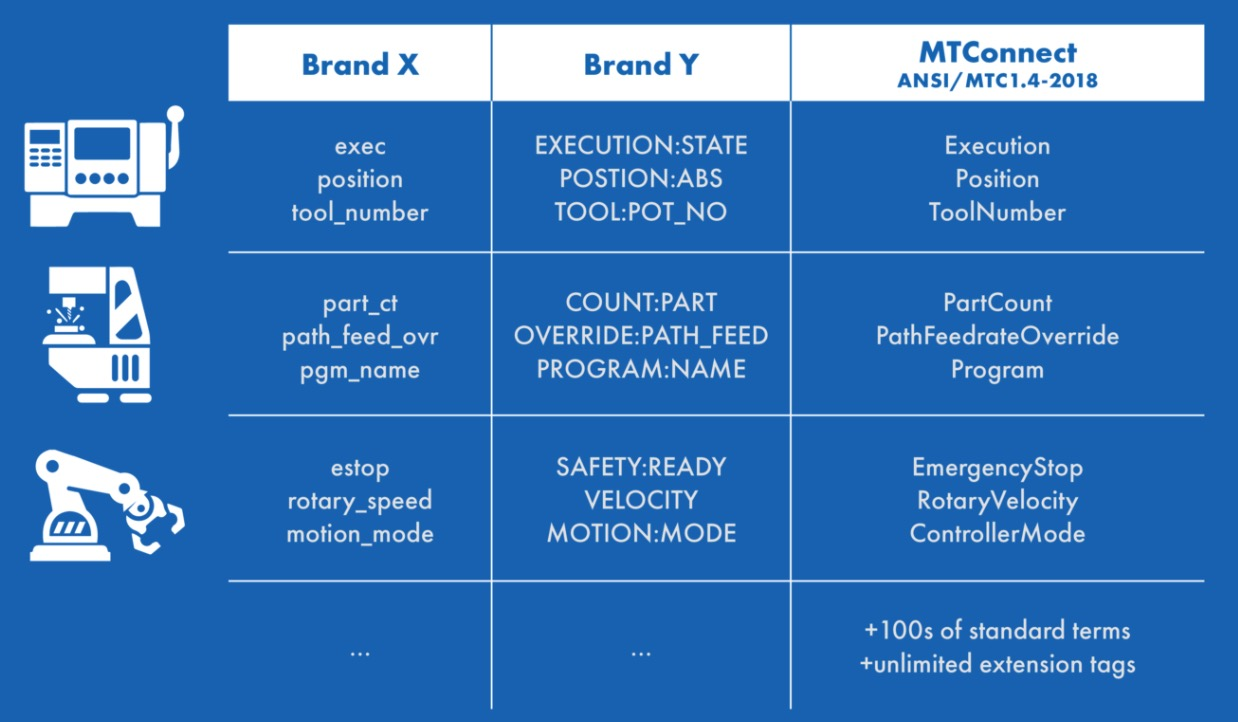
\includegraphics[width=.8\textwidth,angle=0]{figures/mtconnect.jpg}
	\caption{Tabuľka s ukážkou sémantickej výbavy normy MTConnect, zdroj: mtconnect.org.}
\end{figure}

MTConnect poskytuje doménovo-špecifickú slovnú zásobu a dátové modely, je rozšíriteľný a je ho možné kombinovať s inými štandardmi. Vďaka jednotným údajom sa vývojári a integrátori môžu sústrediť skôr na užitočné produktívne výrobné aplikácie než na preklady premenných. MTConnect ale nie je softvér; je to štandard, ktorý definuje dátové štítky a správanie sa softvérového agenta (časti informačného systému pre správu dát). Zdroje údajov zahŕňajú obrábacie stroje, výrobné zariadenia, senzory s ich ovládačmi a ďalší hardvér výrobcu. Aplikácie, ktoré spotrebúvajú údaje MTConnect, poskytujú efektívnejšie operácie a zlepšenú optimalizáciu výroby, čoho výsledkom je zvýšenie produktivity.

Za viac ako 10 rokov od prvého vydania tejto normy sa jej používanie rozšírilo na viac ako 50 000 zariadení od vyše 300 výrobcov vo viac ako 50 krajinách; existuje cez 1000 softvérových riešení implementujúcich túto normu.

\subsection{OMG DDS}

Služba distribúcie údajov (DDS) je middlewarový protokol (softvérová vrstva, ktorá leží medzi operačným systémom a aplikáciami) a štandard API od skupiny Object Management Group (OMG) pre dátovo-centrickú konektivitu. Integruje komponenty systému dohromady a poskytuje dátové pripojenie s nízkou latenciou, extrémnu spoľahlivosť a škálovateľnú architektúru, ktorú potrebujú aplikácie internetu vecí (IoT).

V distribuovanom systéme umožňuje middleware rôznym komponentom systému ľahšiu komunikáciu a zdieľanie údajov. Zjednodušuje sa vývoj distribuovaných systémov tým, že sa vývojári softvéru môžu zamerať skôr na konkrétny účel svojich aplikácií než na detaily spôsobov prenosu informácií medzi aplikáciami a systémami \citep{ddsfoundation}.

\begin{figure}[h!]
	\centering
	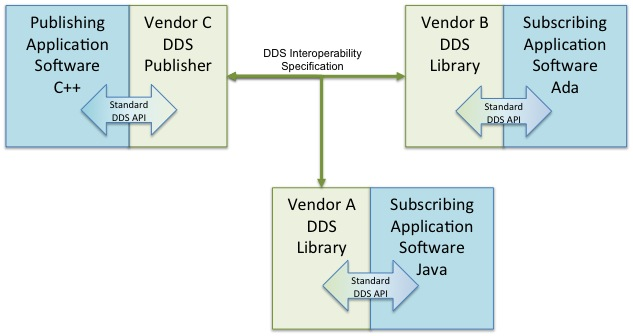
\includegraphics[width=.8\textwidth,angle=0]{figures/omg-dds-interoperability.jpg}
	\caption{Interoperabilita medzi viacerými aplikáciami naprogramovanými odlišnými programovacími jazykmi. Middleware vrstva podľa OMG DDS špecifikácie utvára spoločné rozhranie (API), pomocou ktorého sa rôznorodé aplikácie môžu k sebe navzájom pripájať.}
\end{figure}

%
%%
\Urlmuskip=0mu plus 1mu\relax
\bibliographystyle{spbasic}
\bibliography{refs/control,refs/mathematics,refs/modeling,refs/cfd,refs/lbm,refs/gpu,refs/interaction,refs/interfaces,refs/hci,refs/design,refs/ml,refs/visualization,refs/programming,refs/simulation,refs/ar,refs/vr,refs/online}

%

\end{document}
%%